\documentclass[
    % -- opções da classe memoir --
    12pt,               % tamanho da fonte
    openany,            % capítulos começam em qualquer página (entrega digital, sem páginas em branco)
    oneside,            % para impressão em recto e verso. Oposto a oneside
    a4paper,            % tamanho do papel.
    % -- opções da classe abntex2 --
    chapter=TITLE,      % títulos de capítulos convertidos em letras maiúsculas
    section=TITLE,      % títulos de seções convertidos em letras maiúsculas
    % -- opções do pacote babel --
    english,            % idioma adicional para hifenização
    brazil,             % o último idioma é o principal do documento
    ]{abntex2}

% ---
% PACOTES
% ---

% ---
% Pacotes fundamentais
% ---
\usepackage[T1]{fontenc}        % Selecao de codigos de fonte.
\usepackage[utf8]{inputenc}     % Codificacao do documento (conversão automática dos acentos)
\usepackage{indentfirst}        % Indenta o primeiro parágrafo de cada seção.
\usepackage{color}              % Controle das cores
\usepackage{graphicx}           % Inclusão de gráficos
\usepackage{microtype}          % para melhorias de justificação
\usepackage[absolute]{textpos}

% ---
% PACOTES PARA DIAGRAMAS (TikZ) — usar se necessário no Cap. 2/3
% ---
\usepackage{tikz}
\usetikzlibrary{shapes.geometric, arrows, positioning}

\RequirePackage{helvet}
\renewcommand{\familydefault}{\sfdefault}  % O mais próximo que temos de arial
\usepackage{template/setrem}
% ---

% ---
% Pacotes adicionais
% ---
\usepackage{listings}
\lstset{
  basicstyle=\ttfamily\footnotesize,
  breaklines=true,
  frame=single,
  numbers=left,
  numberstyle=\tiny,
  captionpos=b
}
% ---

% ---
% Pacotes de citações
% ---
\usepackage[alf,abnt-emphasize=bf,abnt-etal-list=2,abnt-etal-cite=2,abnt-etal-text=2,abnt-repeated-title-omit=yes]{abntex2cite} % Citações padrão ABNT
% ---

% ---
% Informações de dados para CAPA e FOLHA DE ROSTO
% ---
\titulo{Robô Atlas: plataforma robótica orientada a objetos para coleta e análise de dados de telemetria}
\autor{ENZO ALLEBRAND, FERNANDO BASTIAN, KERLON RIBEIRO E VICTOR GENZ}
\local{Três de Maio}
\data{2026}
\instituicao{%
    \centering
    \includegraphics[width=\textwidth,keepaspectratio]{template/Cabecalho-Faculdade-2025.png}
}
\tipotrabalho{Projeto Interdisciplinar de Extensão IV}
\preambulo{Relatório do Projeto Interdisciplinar de Extensão IV apresentado ao Curso de Bacharelado em Engenharia de Computação da Faculdade Três de Maio (SETREM), como requisito de avaliação dos componentes curriculares de Estatística, Programação Orientada a Objetos, Banco de Dados e Gerenciamento de Projetos.}
% Confirme os nomes e papéis dos professores antes da versão definitiva.
\orientador[Professores:]{Rodrigo Danielowski, Tiago Luis Cesa Seibel, Jonas Pacheco e Eduardo Mildner}
% ---

% ---
% Configurações de aparência do PDF final
\definecolor{blue}{RGB}{41,5,195}

\makeatletter
\hypersetup{
        pdftitle={\@title},
        pdfauthor={\@author},
        pdfsubject={\imprimirpreambulo},
        pdfcreator={LaTeX with abnTeX2},
        pdfkeywords={abnt}{latex}{abntex}{abntex2}{projeto de pesquisa},
        colorlinks=true,
        linkcolor=black,
        citecolor=black,
        filecolor=black,
        urlcolor=black,
        bookmarksdepth=4
}
\makeatother
% ---

% ----
% Início do documento
% ----
\begin{document}

\selectlanguage{brazil}
\frenchspacing

% ----------------------------------------------------------
% ELEMENTOS PRÉ-TEXTUAIS
% ----------------------------------------------------------
\imprimircapa
\imprimirfolhaderosto

% --- Resumo e palavras-chave ---
\begin{resumo}
O robô Atlas é uma plataforma robótica móvel desenvolvida no curso de Engenharia de Computação da SETREM, operada remotamente e capaz de registrar dados de telemetria durante seu funcionamento. Este trabalho apresenta a consolidação dessa plataforma como uma solução computacional orientada a objetos que integra um aplicativo móvel, desenvolvido em Flutter; comunicação sem fio de curto alcance por Bluetooth Low Energy; serviços embarcados em um Raspberry Pi, coordenados por troca de mensagens sobre o protocolo MQTT; e um serviço de telemetria em nuvem, hospedado na infraestrutura do LARCC, no qual os dados de posição, estado dos motores, nível de bateria e conectividade são persistidos em um banco de dados relacional de séries temporais (PostgreSQL com a extensão TimescaleDB) e disponibilizados por uma interface de programação de aplicações de leitura. Metodologicamente, a pesquisa classifica-se como aplicada, de natureza exploratória e experimental, com abordagem mista, aplicando de forma integrada os fundamentos de Programação Orientada a Objetos, Banco de Dados, Estatística e Gerenciamento de Projetos. Até a presente etapa, encontram-se implementados o aplicativo, os serviços embarcados e o armazenamento e a leitura da telemetria, com a verificação de corretude apoiada em testes automatizados executáveis sem o robô físico. A análise estatística dos dados coletados, voltada à caracterização do desempenho operacional do robô, encontra-se em desenvolvimento e constitui a etapa central do Capítulo de resultados.

\vspace{\onelineskip}
\noindent\textbf{Palavras-chave}: Robótica móvel. Programação orientada a objetos. Telemetria. Banco de dados de séries temporais. Análise de dados.
\end{resumo}

% --- Lista de ilustrações ---
\pdfbookmark[0]{\listfigurename}{lof}
\listoffigures*
\cleardoublepage

% --- Lista de tabelas ---
\pdfbookmark[0]{\listtablename}{lot}
\listoftables*
\cleardoublepage

% --- Lista de abreviaturas e siglas (após as listas, antes do sumário) ---
% Manter em ordem alfabética e restrita às siglas efetivamente usadas no texto.
\begin{siglas}
  \item[API] \textit{Application Programming Interface} (Interface de Programação de Aplicações)
  \item[BLE] \textit{Bluetooth Low Energy} (Bluetooth de Baixa Energia)
  \item[GPIO] \textit{General Purpose Input/Output} (Entrada/Saída de Propósito Geral)
  \item[GPS] \textit{Global Positioning System} (Sistema de Posicionamento Global)
  \item[HTTP] \textit{Hypertext Transfer Protocol} (Protocolo de Transferência de Hipertexto)
  \item[IC] Integração Contínua
  \item[IoT] \textit{Internet of Things} (Internet das Coisas)
  \item[JSON] \textit{JavaScript Object Notation} (Notação de Objetos JavaScript)
  \item[LARCC] \textit{Laboratory of Advanced Research on Cloud Computing}
  \item[MQTT] \textit{Message Queuing Telemetry Transport} (protocolo de mensagens no modelo publicação/assinatura)
  \item[NUS] \textit{Nordic UART Service} (perfil de serviço BLE para comunicação serial)
  \item[POO] Programação Orientada a Objetos
  \item[PWM] \textit{Pulse Width Modulation} (Modulação por Largura de Pulso)
  \item[SGBD] Sistema Gerenciador de Banco de Dados
  \item[SQL] \textit{Structured Query Language} (Linguagem de Consulta Estruturada)
\end{siglas}
\cleardoublepage

% --- Sumário ---
\pdfbookmark[0]{\contentsname}{toc}
\vspace*{138pt}
\tableofcontents*
\cleardoublepage

% ----------------------------------------------------------
% ELEMENTOS TEXTUAIS
% ----------------------------------------------------------
\textual

\chapter*[Introdução]{Introdução}\label{chap:intro}
\addcontentsline{toc}{chapter}{INTRODUÇÃO}

A robótica móvel consolidou-se como um campo de convergência entre computação, eletrônica e controle, no qual sistemas físicos passaram a depender de camadas de software cada vez mais elaboradas para percepção, decisão e comunicação. Em plataformas de pequeno porte, é comum que o robô não opere de forma totalmente autônoma, mas sim por teleoperação, com um operador humano enviando comandos de movimento à distância enquanto o sistema registra continuamente informações sobre o próprio estado -- posição, deslocamento, consumo de energia e conectividade. Esse registro contínuo, conhecido como telemetria, transforma o robô também em uma fonte de dados reais, que, uma vez armazenados e analisados, permitem compreender e validar o comportamento da solução construída.

O tratamento adequado desses dados, porém, não é imediato. À medida que um protótipo evolui de peças isoladas para uma plataforma integrada, cresce a complexidade do software que a sustenta, e com ela a necessidade de organizá-lo segundo princípios que favoreçam a modularidade, a reutilização e a testabilidade -- preocupações centrais da Programação Orientada a Objetos e da Engenharia de Software \cite{sommerville2018}. Do mesmo modo, dados de telemetria só se tornam informação útil quando persistidos em uma estrutura de armazenamento coerente com sua natureza temporal e submetidos a técnicas estatísticas que revelem padrões de comportamento. Esses três aspectos -- estruturação orientada a objetos, armazenamento de dados e análise estatística -- articulam-se sob práticas de gerenciamento de projetos que ordenam o desenvolvimento ao longo do tempo.

É nesse cenário que se insere o robô Atlas, uma plataforma robótica móvel desenvolvida no curso de Engenharia de Computação da SETREM. O robô já opera como um sistema completo, controlado por um aplicativo móvel e capaz de publicar sua telemetria em um serviço de nuvem que a persiste em banco de dados; entretanto, os dados coletados ainda não eram submetidos a nenhuma etapa de análise estatística. Este trabalho parte desse sistema em funcionamento para consolidá-lo como uma solução computacional orientada a objetos e, sobre a base de dados já em operação, estruturar a coleta, o armazenamento e a análise da telemetria, aplicando de forma integrada os quatro componentes curriculares do Projeto Interdisciplinar de Extensão IV.

O presente documento está organizado em três capítulos. O primeiro apresenta a contextualização do estudo, incluindo tema, objetivos, problema, justificativa, metodologia, cronograma e orçamento, sob a orientação da disciplina de Gerenciamento de Projetos. O segundo aborda a fundamentação teórica que sustenta as escolhas de projeto orientado a objetos, de modelagem de banco de dados e de análise estatística, encerrando com a descrição da arquitetura da solução. O terceiro detalha os resultados obtidos até a presente etapa, contemplando o desenvolvimento da solução computacional, a coleta e o armazenamento dos dados e as análises realizadas.

% Capítulo 1 — Projeto (conforme ROTEIRO PIE IV: Justificativa, Objetivos e
% Metodologia, cronograma e orçamento). Ajuste o título do capítulo conforme a
% exigência estrutural final.
\chapter{Projeto} \label{chap:ResearchPlan}

\section{Tema} \label{sec:Theme}
O projeto consiste na consolidação de uma plataforma robótica de controle remoto -- o robô Atlas, desenvolvido no curso de Engenharia de Computação da SETREM -- como uma solução computacional integrada, unindo aplicativo móvel, orquestração embarcada e um serviço de telemetria em nuvem, sob a aplicação conjunta dos fundamentos de Estatística, Programação Orientada a Objetos, Banco de Dados e Gerenciamento de Projetos.

\subsection{Delimitação do Tema} \label{subsec:ThemeDelimitation}
O desenvolvimento e os testes concentram-se no ambiente do curso de Engenharia de Computação da SETREM, em Três de Maio/RS, utilizando a infraestrutura de nuvem do LARCC (\textit{Laboratory of Advanced Research on Cloud Computing}) para a hospedagem do serviço de telemetria. O escopo abrange os três repositórios que compõem o sistema: \texttt{app} (aplicativo Flutter que controla o robô e exibe seu histórico de telemetria), \texttt{orquestrador} (firmware do ESP32, serviços do Raspberry Pi e ingestão/leitura de dados na nuvem) e \texttt{atlas\_ai\_v2} (assistente de voz e rosto animado da plataforma). Este último, embora seja um subsistema majoritariamente independente, integra-se aos demais por meio de uma ponte Bluetooth que pode substituir o ESP32 na recepção dos comandos do aplicativo, e é considerado parte do escopo entregue -- sobretudo como conjunto de exemplos de Programação Orientada a Objetos. A coleta e a análise estatística de dados, contudo, restringem-se à telemetria de operação do robô (posição, motores, bateria e conectividade), não abrangendo o comportamento interno do assistente de voz.

\section{Objetivos} \label{sec:objectives}

\subsection{Objetivo Geral} \label{subsec:general_objective}
Desenvolver, de forma integrada e orientada por boas práticas de gerenciamento de projetos, uma solução computacional orientada a objetos para o robô Atlas, contemplando a coleta de dados reais de telemetria (posição, estado dos motores, bateria e conectividade), seu armazenamento em banco de dados relacional de séries temporais e a aplicação de técnicas estatísticas sobre esses dados para apoiar a validação da solução desenvolvida.

\subsection{Objetivos Específicos} \label{subsec:specific_objectives}
% Guia: lista extraída/adaptada do ROTEIRO PIE IV (Objetivos Específicos, pág. 2).
% Ajustar cada item ao escopo real do projeto do grupo.
Para alcançar o objetivo geral proposto, estabelecem-se os seguintes passos:
\begin{itemize}
    \item Planejar o projeto computacional utilizando fundamentos da disciplina de Gerenciamento de Projetos, definindo escopo, cronograma, responsabilidades e entregas;
    \item Aplicar os princípios da Programação Orientada a Objetos na estruturação do software, promovendo modularidade, reutilização de código e organização lógica da solução;
    \item Realizar a modelagem, criação e manipulação de banco de dados relacionais para o armazenamento dos dados coletados no projeto;
    \item Projetar e implementar mecanismos eficientes de coleta de dados reais, garantindo sua integridade e relevância para posterior análise;
    \item Analisar os dados coletados com base nos fundamentos da Estatística, extraindo informações úteis para a tomada de decisão ou validação da solução desenvolvida;
    \item Construir um protótipo para testes, unindo componentes de automação, controle e software;
    \item Utilizar a infraestrutura do LARCC para o envio, manipulação e visualização de dados;
    \item Divulgar, ao longo do semestre, as atividades desenvolvidas nas redes sociais institucionais, conforme exigência do roteiro (\textit{stories} ou publicação no LinkedIn).
\end{itemize}

\section{Problema} \label{sec:Problem}
O robô Atlas opera hoje majoritariamente por teleoperação: o usuário comanda o movimento pelo aplicativo e a telemetria (posição por GPS, estado dos motores, nível de bateria e estado do Wi-Fi) é publicada via MQTT, replicada para a nuvem e persistida em um banco de dados TimescaleDB. Uma API de leitura publicada recentemente disponibiliza esses dados para visualização no aplicativo -- mapa do trajeto, painel de estado, histórico de eventos -- mas, até o momento, nenhum dos repositórios do projeto implementa qualquer etapa de tratamento estatístico sobre os dados coletados.

Diante disso, o problema de pesquisa define-se como: \textit{de que forma os dados reais de telemetria coletados pelo robô Atlas podem ser tratados estatisticamente para caracterizar o desempenho operacional do robô -- em particular, o consumo de bateria, a utilização dos motores e o deslocamento ao longo do tempo?}

\section{Justificativa} \label{sec:justification}
Do ponto de vista técnico, a justificativa apoia-se no estado atual do sistema: o robô Atlas já opera como uma plataforma completa, integrando aplicativo móvel (Flutter, comunicação Bluetooth Low Energy no padrão Nordic UART Service), firmware embarcado (ESP32) e serviços orquestrados em um Raspberry Pi que se comunicam via protocolo MQTT, com telemetria persistida em nuvem por um banco de dados relacional de séries temporais (TimescaleDB) e disponibilizada por uma API de leitura publicada por meio de túnel Cloudflare. Essa infraestrutura de coleta e armazenamento de dados, já em operação, constitui a base sobre a qual a etapa de análise estatística -- ainda não implementada -- pode ser construída, sem exigir instrumentação adicional do robô.

Do ponto de vista acadêmico, o trabalho possui relevância ao aplicar, de forma interdisciplinar, os quatro componentes curriculares do Projeto Interdisciplinar de Extensão IV. A Programação Orientada a Objetos é exercitada na estruturação dos serviços do robô, com destaque para o roteador de comandos (\texttt{orquestrador/roteador.py}), implementado com o padrão de projeto \textit{Command} \cite{gamma2000} sobre uma classe abstrata, e para a camada de acionamento dos motores (\texttt{motores/acionamento.py}), que abstrai o hardware por meio de outra classe abstrata com implementações concreta (motores de passo reais) e simulada. O Banco de Dados é representado pela modelagem da tabela de telemetria em TimescaleDB e pela camada de consultas parametrizadas da API de leitura. A Estatística, embora ainda pendente de implementação, dispõe de uma base de dados real e crescente para sustentar a análise.

Do ponto de vista social, o projeto mantém sua natureza de extensão, com divulgação periódica das atividades desenvolvidas nas redes sociais institucionais, conforme exigido pelo roteiro do componente curricular.

\section{Metodologia} \label{sec:Methodology}
A pesquisa classifica-se como aplicada, de natureza exploratória e experimental, uma vez que parte de um sistema já em funcionamento -- o robô Atlas -- para investigar, por meio de testes e da coleta de dados reais, o comportamento e o desempenho da solução desenvolvida. A abordagem é mista: qualitativa na descrição da arquitetura, das decisões de projeto orientado a objetos e da integração entre os subsistemas; e quantitativa na análise dos dados numéricos de telemetria (posição, velocidade, nível de bateria, estado de conectividade) armazenados no banco de dados.

\subsection{Procedimentos Metodológicos} \label{subsec:methodological_procedures}
O desenvolvimento é conduzido de forma incremental e iterativa \cite{prikladnicki2014} em três repositórios versionados independentemente (\texttt{app}, \texttt{orquestrador} e \texttt{atlas\_ai\_v2}), com controle de versão via Git e revisão automatizada de dependências (Dependabot). A verificação de corretude apoia-se em testes automatizados, prática central da garantia de qualidade de software \cite{sommerville2018}: o roteador de comandos e a camada de acionamento dos motores do \texttt{orquestrador} somam dezenas de testes unitários executáveis sem hardware físico -- sem broker MQTT, sem Raspberry Pi e sem motores conectados --, a API de leitura da telemetria possui suíte própria de testes cobrindo cabeçalhos de segurança e consultas, e o subsistema \texttt{atlas\_ai\_v2} mantém integração contínua via GitHub Actions, executando sua suíte de testes em múltiplas versões do Python e sistemas operacionais a cada alteração. O aplicativo móvel utiliza entrega contínua (Shorebird), permitindo atualizações incrementais sem reinstalação. Essas práticas sustentam a rastreabilidade entre implementação e relatório exigida pelas diretrizes deste trabalho.

\subsection{Coleta e Análise de Dados} \label{subsec:data_collection}
A coleta de dados ocorre continuamente durante a operação do robô: os serviços do Raspberry Pi publicam, via protocolo MQTT, o estado dos motores, a posição obtida por GPS, o nível de bateria e o estado da conexão Wi-Fi; esses tópicos são espelhados para um broker remoto e persistidos por um serviço de ingestão em uma tabela única do TimescaleDB, particionada por tempo (\textit{hypertable}), com o payload de cada tipo de telemetria armazenado em formato \texttt{JSONB}. O uso de uma tabela genérica, em vez de uma tabela por tipo de dado, evita migração de esquema a cada nova categoria de telemetria introduzida.

Até o momento, esses dados são consumidos apenas para fins operacionais -- visualização do trajeto e do estado do robô no aplicativo, por meio da API de leitura -- sem qualquer etapa de análise estatística. Esta é a principal lacuna identificada no sistema atual e o ponto de partida para o Capítulo~\ref{chap:Results} deste relatório. Para caracterizar o desempenho operacional do robô, prevê-se a aplicação de medidas de tendência central e de dispersão (média, mediana e desvio padrão) sobre variáveis como o nível de bateria e a velocidade dos motores, e de técnicas de análise de séries temporais para descrever a evolução dessas variáveis e do deslocamento ao longo do tempo. Em coerência com a diretriz de rastreabilidade adotada neste trabalho, nenhum resultado de análise será descrito antes de sua execução efetiva sobre os dados reais coletados.

\section{Cronograma de Atividades} \label{sec:schedule_activities_table}
% Guia: cronograma alinhado às datas do ROTEIRO PIE IV (15/08 a 19/12/2026).
% Ajustar as atividades internas do grupo mantendo os marcos de entrega oficiais.
O desenvolvimento da pesquisa respeitará as datas avaliativas estipuladas para a disciplina, conforme a \autoref{tab:cronograma}.

\begin{table}[htb]
\centering
\caption{Cronograma de Atividades do Projeto de Extensão}
\label{tab:cronograma}
\begin{tabular}{|p{7.5cm}|c|c|c|c|}
\hline
\textbf{Atividade} & \textbf{Set.} & \textbf{Out.} & \textbf{Nov.} & \textbf{Dez.} \\ \hline
Definição de tema, escopo e levantamento de requisitos & X & & & \\ \hline
Modelagem do banco de dados e planejamento do projeto & X & & & \\ \hline
Desenvolvimento da solução orientada a objetos & & X & & \\ \hline
Implementação da coleta de dados e integração & & X & X & \\ \hline
Análise estatística dos dados coletados & & & X & \\ \hline
Escrita do relatório final e ajustes documentais & & & X & X \\ \hline
Apresentação final do projeto (bancas) & & & & X \\ \hline
\end{tabular}
\fonte{Elaborado pelos autores (2026).}
\end{table}

\section{Orçamento} \label{sec:budget}
A \autoref{tab:orcamento} relaciona os principais itens de hardware que compõem o protótipo do robô Atlas, base física sobre a qual o software e a coleta de dados são desenvolvidos. A infraestrutura de nuvem utilizada para a telemetria é fornecida pelo LARCC, sem custo direto para o grupo, assim como as ferramentas de software empregadas, todas de código aberto ou gratuitas para uso acadêmico. Os valores unitários e totais serão confirmados pelo grupo a partir das notas fiscais e cotações efetivas dos componentes já adquiridos.

\begin{table}[htb]
\centering
\caption{Orçamento Previsto para o Desenvolvimento do Projeto}
\label{tab:orcamento}
\begin{tabular}{|p{7.2cm}|c|r|}
\hline
\textbf{Item} & \textbf{Quantidade} & \textbf{Valor Total Estimado (R\$)} \\ \hline
Raspberry Pi (computador embarcado) & 1 & a confirmar \\ \hline
Microcontrolador ESP32 (ponte BLE) & 1 & a confirmar \\ \hline
Motores de passo & 2 & a confirmar \\ \hline
Drivers de motor de passo TMC2209 & 2 & a confirmar \\ \hline
Módulo receptor GPS & 1 & a confirmar \\ \hline
Bateria e sistema de alimentação & 1 & a confirmar \\ \hline
Estrutura/chassi e componentes mecânicos & 1 & a confirmar \\ \hline
Infraestrutura de nuvem (LARCC) & 1 & sem custo \\ \hline
\textbf{Total} & \textbf{--} & \textbf{a confirmar} \\ \hline
\end{tabular}
\fonte{Elaborado pelos autores (2026).}
\end{table}

% Capítulo 2 — Fundamentação Teórica (conforme ROTEIRO PIE IV).
\chapter{Fundamentação Teórica}\label{chap:FundamentacaoTeorica}

Este capítulo apresenta os fundamentos teóricos que sustentam as decisões de projeto adotadas no desenvolvimento do robô Atlas, organizados segundo os quatro componentes curriculares do Projeto Interdisciplinar de Extensão IV: Programação Orientada a Objetos, Modelagem de Banco de Dados, Estatística Aplicada à Análise de Dados e Gerenciamento de Projetos, encerrando com a descrição da arquitetura da solução que integra esses fundamentos na prática.

\section{Revisão da Literatura} \label{sec:revisao_literatura}
A fundamentação deste trabalho apoia-se em obras consolidadas de cada um dos campos que o projeto integra. No campo do software, a Programação Orientada a Objetos e os padrões de projeto que dela derivam são tratados a partir de referências clássicas da área \cite{deitel2016,gamma2000}, enquanto as práticas de engenharia e de qualidade de software que orientam o desenvolvimento remetem à literatura de Engenharia de Software \cite{sommerville2018}. No campo do armazenamento, a modelagem relacional e os sistemas gerenciadores de banco de dados são fundamentados em literatura consagrada da área \cite{elmasri2011}. No campo da análise, os fundamentos de Estatística descritiva e de análise de séries temporais provêm de referências amplamente adotadas no ensino de engenharia \cite{bussab2017,morettin2018}. Por fim, as práticas de condução do projeto ao longo do semestre baseiam-se na literatura de métodos ágeis de desenvolvimento de software \cite{prikladnicki2014}.

Além dessas bases teóricas, o projeto situa-se no encontro de três eixos tecnológicos, decorrentes diretamente das soluções já empregadas: a robótica móvel teleoperada e os protocolos de comunicação de curto alcance para controle remoto, representados pelo uso de Bluetooth Low Energy no padrão \textit{Nordic UART Service}; as arquiteturas orientadas a mensagens, aplicadas na comunicação entre os serviços embarcados por meio do protocolo MQTT; e os bancos de dados de séries temporais aplicados à telemetria de sistemas embarcados, materializados na escolha do TimescaleDB. As seções seguintes desenvolvem cada um desses fundamentos e encerram com a descrição da arquitetura que os integra.

\section{Programação Orientada a Objetos} \label{sec:poo}
A Programação Orientada a Objetos organiza um sistema em classes, que encapsulam estado (atributos) e comportamento (métodos) atrás de uma interface pública \cite{deitel2016}. Quatro princípios sustentam o paradigma: \textbf{encapsulamento}, que oculta os detalhes internos de uma classe e restringe o acesso direto ao seu estado; \textbf{abstração}, que define o que uma classe faz -- por meio de classes ou interfaces abstratas -- sem especificar como; \textbf{herança}, que permite que uma subclasse reutilize e especialize o comportamento de uma superclasse; e \textbf{polimorfismo}, que permite que um mesmo ponto de chamada produza comportamentos distintos conforme a subclasse concreta envolvida, resolvida em tempo de execução.

No repositório \texttt{orquestrador}, esses princípios aparecem de forma concreta em dois pontos. O roteamento de comandos (\texttt{pi/services/orquestrador/.../roteador.py}) segue o padrão de projeto \textit{Command} \cite{gamma2000}: a classe abstrata \texttt{ComandoRoteavel} declara o método abstrato \texttt{rotear()}, implementado por cinco subclasses concretas -- para comandos de motor, de voz, de parada de emergência, de provisionamento de Wi-Fi e de validação de rota segura --, cada uma responsável por um tipo de comando recebido do aplicativo. A função pública de despacho não conhece a subclasse concreta do outro lado: ela invoca \texttt{rotear()} polimorficamente, e o comportamento correto é resolvido conforme o tipo do comando recebido. Esse desenho torna a adição de um novo tipo de comando uma questão de criar uma subclasse nova, sem alterar a lógica de despacho existente.

O segundo ponto é a camada de acionamento dos motores (\texttt{motores/acionamento.py}), em que a classe abstrata \texttt{Acionamento} isola o serviço de motores do hardware concreto: a subclasse \texttt{AcionamentoStepper} traduz comandos de velocidade em sinais PWM para os drivers dos motores de passo reais, enquanto a subclasse \texttt{AcionamentoSimulado} apenas registra o que teria sido executado, permitindo desenvolver e testar o serviço sem o robô fisicamente montado. O serviço depende apenas da interface abstrata, nunca de uma implementação concreta específica -- uma aplicação do princípio de inversão de dependência.

O subsistema \texttt{atlas\_ai\_v2} (assistente de voz e rosto animado da Atlas) concentra os exemplos mais completos de POO do projeto: uma hierarquia de herança e polimorfismo clássicos, em que uma classe base imutável de evento (\texttt{core/events.py::Event}) é especializada em oito subclasses de evento (mensagem do usuário, início e fim de fala, ocorrência de erro, entre outras), despachadas por verificação de tipo em tempo de execução; o padrão de projeto \textit{Factory Method} \cite{gamma2000}, na escolha do cliente de modelo de linguagem e do motor de síntese de voz a instanciar conforme a configuração; o padrão \textit{Decorator} \cite{gamma2000}, em que uma classe envolve um motor de voz primário e um de reserva atrás da mesma interface, promovendo tolerância a falhas; e abstração por tipagem estrutural (\textit{duck typing}), via \texttt{typing.Protocol}, para as interfaces de cliente de linguagem e de motor de voz -- uma forma de abstração distinta da herança nominal clássica (\texttt{class X(Base)}), útil para diferenciar os dois casos quando a disciplina exigir.

\section{Modelagem de Banco de Dados} \label{sec:banco_dados}
O modelo relacional organiza os dados em relações (tabelas) compostas por atributos, sobre as quais operam uma linguagem de consulta declarativa (SQL) e mecanismos de indexação que sustentam o desempenho das consultas \cite{elmasri2011}. O modelo de dados adotado para a telemetria do robô Atlas é relacional, sobre o sistema gerenciador PostgreSQL, com a extensão TimescaleDB para lidar eficientemente com séries temporais. Em vez de normalizar os dados em uma tabela por tipo de telemetria, o sistema persiste todos os tipos -- posição por GPS, estado dos motores, nível de bateria, estado do Wi-Fi -- em uma única tabela genérica (\texttt{telemetria}), com colunas de carimbo de tempo (\texttt{ts}), tipo (\texttt{tipo}), tópico de origem (\texttt{topico}) e o restante do dado em uma coluna semiestruturada (\texttt{payload}, do tipo \texttt{JSONB}). Essa tabela é transformada em uma \textit{hypertable} pelo TimescaleDB, que a particiona automaticamente por tempo, e um índice composto em (\texttt{tipo}, \texttt{ts} decrescente) sustenta as duas consultas mais frequentes: a última leitura de cada tipo e a evolução de um tipo ao longo do tempo.

Essa escolha de modelagem prioriza a flexibilidade sobre a normalização estrita: adicionar um novo tipo de dado -- por exemplo, um novo sensor -- não exige migração de esquema, apenas um novo valor para a coluna \texttt{tipo} e a estrutura livre do respectivo \texttt{payload}.

Sobre esse armazenamento, uma API de leitura (\texttt{orquestrador/cloud/api}, construída com o \textit{framework} FastAPI) expõe a telemetria por HTTP, autenticada por token, com um usuário de banco de dados restrito apenas à operação \texttt{SELECT} -- separando o caminho de escrita, exclusivo do serviço de ingestão, do caminho de leitura, exposto à internet por um túnel Cloudflare. As consultas dessa API ilustram técnicas de modelagem e otimização relevantes: o operador \texttt{DISTINCT ON} do PostgreSQL, para obter o último valor de cada tipo em uma única consulta; a função \texttt{time\_bucket()} do TimescaleDB, para agregação temporal que aproveita a própria partição da \textit{hypertable} em vez de uma leitura linha a linha; paginação por cursor de tempo, em vez de deslocamento (\texttt{OFFSET}), para evitar que registros novos desloquem páginas já lidas; e validação estrita dos parâmetros que precisam ser interpolados diretamente no texto da consulta (o nome do campo agregado e o intervalo de agregação, que a sintaxe do SQL não aceita como parâmetro), como salvaguarda contra injeção de SQL.

\section{Estatística Aplicada à Análise de Dados} \label{sec:estatistica}
Não foi identificado, até o momento, nenhum código de análise estatística em execução sobre os dados de telemetria do robô: não há uso de bibliotecas como \texttt{pandas}, \texttt{numpy} ou \texttt{statistics} para esse fim em nenhum dos três repositórios do projeto -- o uso de \texttt{numpy} encontrado em \texttt{atlas\_ai\_v2} está restrito ao processamento de áudio e à renderização gráfica do rosto animado, sem relação com os dados de telemetria. Esta é a lacuna mais relevante identificada no levantamento do projeto, e a que responde mais diretamente ao problema de pesquisa formulado no Capítulo 1.

A tabela \texttt{telemetria} do TimescaleDB, descrita na Seção~\ref{sec:banco_dados}, é a fonte de dados real sobre a qual essa análise será construída, em resposta ao problema de pesquisa formulado no Capítulo~\ref{chap:ResearchPlan}: caracterizar o desempenho operacional do robô. A fundamentação teórica desta análise sustenta-se em dois conjuntos de técnicas. O primeiro é a Estatística descritiva, que resume um conjunto de dados por medidas de tendência central -- como a média e a mediana -- e por medidas de dispersão -- como o desvio padrão --, e que comunica sua distribuição por meio de representações gráficas, como o histograma \cite{bussab2017}; essas medidas serão aplicadas a variáveis como o nível de bateria e a velocidade dos motores. O segundo é a análise de séries temporais, adequada a dados indexados no tempo, como os coletados continuamente pela telemetria do robô, e voltada a descrever tendências e variações de uma variável ao longo do tempo \cite{morettin2018}; será empregada para caracterizar a evolução do consumo de energia e do deslocamento durante a operação. Em coerência com a diretriz de rastreabilidade adotada neste trabalho, nenhum resultado de análise estatística será descrito antes de sua execução efetiva sobre os dados reais coletados.

\section{Arquitetura da Solução} \label{sec:arquitetura}
A arquitetura do robô Atlas divide-se em três frentes fisicamente distintas -- um aplicativo móvel, um conjunto de serviços embarcados e um back-end em nuvem --, que se comunicam por protocolos diferentes conforme a distância física entre as partes e a confiabilidade exigida em cada trecho, como ilustra a \autoref{fig:diagrama_blocos}.

O aplicativo (Flutter, Android e iOS) envia comandos de movimento e de planejamento de rota ao robô por Bluetooth Low Energy, no padrão \textit{Nordic UART Service}. Um firmware embarcado no ESP32 recebe esses comandos pela característica BLE, valida sua estrutura como JSON e os repassa por uma conexão serial (115200 bauds) ao Raspberry Pi, sem interpretar seu conteúdo. No Raspberry Pi, um barramento MQTT local (\textit{broker} Mosquitto) desacopla cinco serviços Python independentes: o serviço que ingere a linha serial publica o comando cru; o serviço orquestrador o interpreta, por meio do roteador de comandos descrito na \autoref{sec:poo}, e o redistribui para os serviços responsáveis por motores, Wi-Fi e GPS. Cada um desses serviços publica de volta seu próprio estado, que o orquestrador espelha sob um conjunto de tópicos de telemetria.

Esses tópicos de telemetria são replicados, por uma ponte do Mosquitto, para um \textit{broker} remoto hospedado em uma máquina virtual na infraestrutura do LARCC, onde um serviço de ingestão os persiste no banco de dados TimescaleDB descrito na \autoref{sec:banco_dados}. Uma API de leitura, publicada por um túnel Cloudflare, permite que o aplicativo -- de qualquer lugar, com o robô ligado ou desligado -- consulte esse histórico, fechando o ciclo entre a operação do robô e sua visualização.

\begin{figure}[htb]
\centering
\caption{Diagrama de blocos da arquitetura do robô Atlas.}
\label{fig:diagrama_blocos}
\resizebox{\textwidth}{!}{%
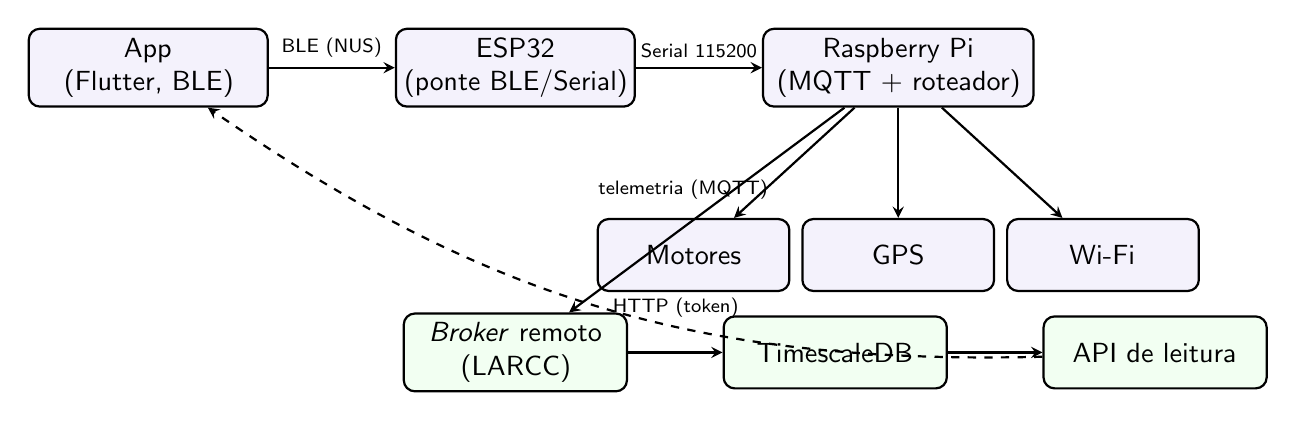
\begin{tikzpicture}[
    box/.style={rectangle, draw=black, thick, fill=blue!5, minimum height=2.6em, text centered, rounded corners, text width=2.8cm},
    cloudbox/.style={box, fill=green!5},
    arrow/.style={thick,->,>=stealth},
    lbl/.style={font=\scriptsize, midway, above}
]
% Caminho físico: app -> ESP32 -> Raspberry Pi -> serviços locais
\node (app) [box] {App\\(Flutter, BLE)};
\node (esp32) [box, right=1.6cm of app] {ESP32\\(ponte BLE/Serial)};
\node (pi) [box, right=1.6cm of esp32, text width=3.2cm] {Raspberry Pi\\(MQTT + roteador)};
\node (motores) [box, below=1.4cm of pi, xshift=-2.6cm, text width=2.2cm] {Motores};
\node (gps) [box, below=1.4cm of pi, text width=2.2cm] {GPS};
\node (wifi) [box, below=1.4cm of pi, xshift=2.6cm, text width=2.2cm] {Wi-Fi};

\draw [arrow] (app) -- node[lbl] {BLE (NUS)} (esp32);
\draw [arrow] (esp32) -- node[lbl] {Serial 115200} (pi);
\draw [arrow] (pi) -- (motores);
\draw [arrow] (pi) -- (gps);
\draw [arrow] (pi) -- (wifi);

% Caminho de ida: telemetria até o banco
\node (broker) [cloudbox, below=2.6cm of esp32, text width=2.6cm] {\textit{Broker} remoto (LARCC)};
\node (db) [cloudbox, right=1.2cm of broker, text width=2.6cm] {TimescaleDB};
\node (api) [cloudbox, right=1.2cm of db, text width=2.6cm] {API de leitura};

\draw [arrow] (pi) -- node[lbl, xshift=-0.3cm] {telemetria (MQTT)} (broker);
\draw [arrow] (broker) -- (db);
\draw [arrow] (db) -- (api);

% Caminho de volta: API até o app
\draw [arrow, dashed] (api) to[bend left=18] node[midway, right, font=\scriptsize] {HTTP (token)} (app);
\end{tikzpicture}%
}
\fonte{Elaborado pelos autores (2026), a partir do código dos repositórios \texttt{app} e \texttt{orquestrador}.}
\end{figure}

\section{Gerenciamento de Projetos} \label{sec:gerenciamento_projetos}
O Gerenciamento de Projetos fornece as práticas que estruturam a condução do trabalho ao longo do semestre -- definição de escopo, cronograma, papéis e entregas --, complementando os demais componentes curriculares, que tratam do que é construído. O grupo adota um referencial ágil, apoiado no método Kanban, cuja ênfase está na visualização do fluxo de trabalho por meio de um quadro de tarefas, na limitação do trabalho em andamento e na entrega contínua de incrementos \cite{prikladnicki2014}. Essa escolha é coerente com a natureza incremental do desenvolvimento e com o tamanho reduzido da equipe: em vez de ciclos fechados com papéis rígidos, o Kanban organiza um fluxo contínuo de pequenas tarefas -- alinhado ao versionamento por repositórios já em uso --, cujas entregas se conectam aos marcos avaliativos apresentados na \autoref{tab:cronograma} (\autoref{sec:schedule_activities_table}, Capítulo~\ref{chap:ResearchPlan}). A adoção crescente de métodos ágeis é reconhecida também na literatura de Engenharia de Software \cite{sommerville2018}.

Do ponto de vista técnico, o próprio desenvolvimento do sistema já incorpora práticas de gerenciamento reconhecidas: os três repositórios são versionados de forma independente, com controle de dependências automatizado (Dependabot), e o repositório \texttt{atlas\_ai\_v2} mantém integração contínua (GitHub Actions) executando sua suíte de testes a cada alteração. Essas práticas relacionam-se a conceitos consolidados de gestão de configuração e de garantia de qualidade em projetos de software \cite{sommerville2018}.

% Capítulo 3 — Resultados (conforme ROTEIRO PIE IV).
% NOTA: conforme o cronograma da disciplina, o Capítulo 3 é desenvolvido a partir
% de 24/10. Os parágrafos abaixo descrevem, de forma honesta, o que cada seção
% apresentará -- sem antecipar resultados que ainda não foram produzidos. Nenhum
% número ou análise deve ser inserido antes de sua execução efetiva sobre os
% dados reais coletados.
\chapter{Resultados}\label{chap:Results}

Este capítulo apresenta os resultados obtidos até a presente etapa do desenvolvimento do projeto, organizados do protótipo físico à análise dos dados coletados: o hardware do robô, a solução computacional orientada a objetos, o banco de dados de telemetria, a coleta e a análise estatística dos dados, a integração entre as partes e as evidências de extensão exigidas pelo componente curricular.

% ---------------------------------------------------------------------------
\section{Desenvolvimento do Hardware / Protótipo} \label{sec:dev_hardware}
% ---------------------------------------------------------------------------
% Guia: descrever o protótipo físico (componentes, esquema de ligação, fotos),
% análogo ao Cap. 3 do PIE III. Inserir fotografias do robô em img/.
Esta seção descreve o protótipo físico do robô Atlas -- estrutura mecânica, computador embarcado (Raspberry Pi), microcontrolador ESP32, motores de passo com seus respectivos \textit{drivers}, módulo GPS e sistema de alimentação -- e o esquema de ligação entre esses componentes. \textit{(Seção em desenvolvimento: incluir fotografias e o diagrama de ligações do protótipo montado.)}

% ---------------------------------------------------------------------------
\section{Desenvolvimento da Solução Orientada a Objetos} \label{sec:dev_software}
% ---------------------------------------------------------------------------
% Guia: descrever as principais classes/módulos implementados e os padrões de
% projeto aplicados, retomando a fundamentação da Seção~\ref{sec:poo}.
Esta seção detalha a implementação da solução computacional, retomando na prática os conceitos apresentados na \autoref{sec:poo}: as principais classes e módulos dos repositórios \texttt{orquestrador} e \texttt{atlas\_ai\_v2}, os padrões de projeto aplicados e a organização em camadas que separa a lógica pura do acesso a hardware, permitindo a verificação por testes automatizados. \textit{(Seção em desenvolvimento.)}

\subsection{Modelagem de Classes} \label{subsec:modelagem_classes}
% Guia: apresentar o diagrama de classes das partes centrais (roteador de
% comandos, camada de acionamento dos motores, hierarquia de eventos).
Apresenta-se aqui o diagrama das classes centrais da solução -- a hierarquia do roteador de comandos, a camada de acionamento dos motores e a hierarquia de eventos do assistente --, evidenciando as relações de herança e a resolução polimórfica descritas na fundamentação teórica. \textit{(Seção em desenvolvimento: inserir o diagrama de classes.)}

% ---------------------------------------------------------------------------
\section{Banco de Dados} \label{sec:dev_banco}
% ---------------------------------------------------------------------------
% Guia: modelo implementado, SGBD utilizado, script de criação da tabela.
Esta seção apresenta o modelo de dados efetivamente implementado -- a tabela de telemetria em PostgreSQL/TimescaleDB descrita na \autoref{sec:banco_dados} --, o \textit{script} de criação, a transformação em \textit{hypertable} e os índices que sustentam as consultas mais frequentes. \textit{(Seção em desenvolvimento: incluir o script de criação e exemplos de consulta.)}

% ---------------------------------------------------------------------------
\section{Coleta de Dados} \label{sec:coleta_dados}
% ---------------------------------------------------------------------------
% Guia: como os dados reais são coletados, volume obtido e integração com o LARCC.
Esta seção descreve o mecanismo de coleta de dados reais em operação: a publicação da telemetria pelos serviços do Raspberry Pi, seu espelhamento para o \textit{broker} remoto hospedado no LARCC e sua persistência no banco de dados. Serão relatados o período de coleta e o volume de registros efetivamente obtidos até a análise. \textit{(Seção em desenvolvimento: informar o volume de dados coletados.)}

% ---------------------------------------------------------------------------
\section{Análise Estatística dos Dados} \label{sec:analise_estatistica}
% ---------------------------------------------------------------------------
% Guia: tabelas/gráficos das análises realizadas e a interpretação dos resultados.
% Aplicar as técnicas fundamentadas na Seção~\ref{sec:estatistica}: estatística
% descritiva (Bussab e Morettin) e séries temporais (Morettin e Toloi).
Esta seção apresenta a análise estatística dos dados coletados, voltada à caracterização do desempenho operacional do robô. Serão aplicadas as técnicas fundamentadas na \autoref{sec:estatistica} -- medidas de tendência central e de dispersão \cite{bussab2017} sobre variáveis como o nível de bateria e a velocidade dos motores, e análise de séries temporais \cite{morettin2018} sobre a evolução do consumo de energia e do deslocamento --, acompanhadas das tabelas, dos gráficos e da interpretação correspondente. \textit{(Seção em desenvolvimento: os resultados serão inseridos após a execução da análise sobre os dados reais.)}

% ---------------------------------------------------------------------------
\section{Integração entre Hardware e Software} \label{sec:integracao}
% ---------------------------------------------------------------------------
% Guia: fluxo completo de ponta a ponta (app -> hardware -> nuvem -> banco -> análise).
Esta seção descreve o funcionamento integrado da solução, do comando enviado pelo aplicativo até a visualização e a análise dos dados na nuvem, percorrendo o caminho detalhado na \autoref{sec:arquitetura} e evidenciando como as partes desenvolvidas separadamente operam em conjunto. \textit{(Seção em desenvolvimento.)}

% ---------------------------------------------------------------------------
\section{Conexão com a Comunidade} \label{sec:comunidade}
% ---------------------------------------------------------------------------
% Guia (exigência do ROTEIRO PIE IV): fotografias, formulários de pesquisa,
% entrevistas, feedback da instituição parceira e registro das publicações nas
% redes sociais (stories/LinkedIn) exigidas pelo componente curricular.
Esta seção reúne as evidências de extensão do projeto, conforme exigido pelo componente curricular: registros de campo, eventual coleta de \textit{feedback} de representantes da instituição parceira e o comprovante das publicações realizadas nas redes sociais institucionais (\textit{stories} no Instagram, marcando o perfil \texttt{@comp.setrem}, ou publicação no LinkedIn). \textit{(Seção em desenvolvimento: anexar os comprovantes das publicações e demais evidências.)}

\chapter{Considerações Finais}\label{chap:conclusao}

% NOTA: as considerações finais serão consolidadas após o Capítulo 3. O texto
% abaixo retoma o objetivo e o estado atual do projeto sem antecipar resultados
% ainda não produzidos -- completar quando a análise estiver concluída.

Este trabalho teve como objetivo consolidar o robô Atlas como uma solução computacional orientada a objetos voltada à coleta, ao armazenamento e à análise de dados reais de telemetria, aplicando de forma integrada os fundamentos de Programação Orientada a Objetos, Banco de Dados, Estatística e Gerenciamento de Projetos.

Até a presente etapa, encontram-se implementados o aplicativo de controle, os serviços embarcados de orquestração, o armazenamento da telemetria em banco de dados de séries temporais e a interface de leitura desses dados, com a corretude apoiada em testes automatizados executáveis sem o robô físico. \textit{(A completar: retomar os principais resultados do \autoref{chap:Results}.)}

Quanto aos objetivos específicos, \textit{(a completar: indicar quais foram plenamente atendidos e quais permanecem em andamento -- em especial a etapa de análise estatística)}.

Reconhecem-se, ainda, as limitações já apontadas no \autoref{chap:Results}, com destaque para a análise estatística dos dados coletados, principal lacuna identificada e foco da etapa final do projeto.

Como trabalhos futuros, indicam-se a continuidade da coleta e da análise de dados, o refinamento das técnicas estatísticas aplicadas, a evolução da solução de software e a maior integração entre o assistente de voz (\texttt{atlas\_ai\_v2}) e o restante da plataforma, além dos demais itens identificados ao longo do desenvolvimento.


% ----------------------------------------------------------
% ELEMENTOS PÓS-TEXTUAIS
% ----------------------------------------------------------
\postextual

% Referências bibliográficas
\bibliography{bib/bibliography}

% Anexos / Apêndices
% NOTA: inserir aqui o conteúdo dos anexos quando disponível (ex.: código-fonte,
% fotografias do protótipo/hardware, formulários de pesquisa, prints de stories/
% publicações no Instagram/LinkedIn exigidos pelo roteiro, e demais evidências de
% extensão). Mantido comentado para não gerar uma página "ANEXO" vazia.
% \begin{anexosenv}
% \phantomsection
% \chapter*{\MakeUppercase{\appendixname}}
% \addcontentsline{toc}{chapter}{\MakeUppercase{\appendixname}}
% % ... conteúdo do anexo aqui ...
% \end{anexosenv}

\end{document}
